\documentclass[specialist, 12pt, href]{article}
\usepackage[utf8]{inputenc}
\usepackage[russian]{babel}
\usepackage[T2A]{fontenc}
\usepackage{indentfirst}
\usepackage{caption}
\usepackage{latexsym,amssymb,amsthm}
\usepackage{amsfonts}
\usepackage{amsmath}
\usepackage{graphicx}
\usepackage{subfigure}

\usepackage[a4paper, includefoot,
            left=2cm, right=2cm,
            top=2cm, bottom=2cm,
            headsep=1cm, footskip=1cm]{geometry}

\usepackage{hyperref}
\setcounter{tocdepth}{2}
\allowdisplaybreaks[4]

\linespread{1.2}
\title{Boosting}
\author{Зиннатулина Белла}
\date{}

\begin{document}
\maketitle

\section{Введение}

В сфере анализа данных существует великое множество методов решения уже классических задач регрессии и классификации. Однако, при всем многообразии и сложности моделей, зачастую алгоритмы либо теряют обобщающую способность, т.е. переобучаются, либо не достигают желаемого качества восстановления зависимости. Возникает вопрос о решении проблемы. В работе Валианта “A theory of the learnable” 1984 года были представлены теоретические основы PAC-модели приближенно правильного обучения (Probably Approximately Correct), где рассматривалась возможность улучшить алгоритм классификации с помощью нескольких слабых классификаторов. В 1989 году Шапир первым придумал такой алгоритм с полиномиальной сложностью, а через год Фрейнд разработал более эффективную реализацию, которая стала основой алгоритма AdaBoost, представленного в 1995 году Шапиром и Фрейндом уже вместе. 

\section{Постановка задачи}

Рассматривается задача обучения $<X,Y, f, X^{n}>$, где  \begin{itemize}
  \item $X$ --- пространство объектов, $Y$ --- можество ответов, 
  \item $f: X \rightarrow Y$ --- неизвестная целевая зависимость, 
  \item $X^{n} = (x_1,\dots,x_{n})$ --- обучающая выборка,
  \item $Y^{n} = (y_1,\dots, y_{n})$ --- вектор ответов на обучающих объектах, где $y_i = f(x_i)$,
  \item $a(x) = C(b(x))$ --- алгоритм, аппроксимирующий целевую зависимость $f$ на всем множестве $X$,
  \item $b:X \rightarrow R$ --- базовый алгоритм,
  \item $C:R \rightarrow Y$ --- решающее правило,
  \item $R$ --- пространство оценок.
  
\end{itemize}

В случае решения задачи классификации значением $b(x)$ может являться вероятность принадлежности объекта $x$ классу, котоое решающее правило $C$ переводит в номер класса.

\textbf{Определение.} Композиция базовых алгоритмов $b_1,\dots, b_T \in \mathcal{B}$ имеет вид

 $a(x) = C(F(b_1(x),\dots,b_T(x))),$ где $F:R^T \rightarrow R$ --- корректирующая операция.

\textbf{Главная идея} --- построить композицию простых алгоритмов, где каждый новый алгоритм исправляет ошибки уже построенной композиции.

\textbf{Пример 1.} Рассмотрим задачу регрессии. В этом случае $C(b) \equiv b, Y = \mathbb{R}, R \equiv \mathbb{R}$, использовать решающее правило смысла нет. 

Пусть $F(b_1(x),\dots,b_T(x)) = \sum\limits_{t = 1}^{T}{b_t(x)}, x \in X$. 

Обучим простой алгоритм $b_1(x) = \underset{b \in \mathcal{B}}{\arg\min} \frac{1}{n}\sum\limits_{i = 1}^{n}{(b(x_i) - y_i)^2}$. Добавим алгоритм $b_2$, исправляющий ошибки $b_1$: $b_1(x_i) + b_2(x_i) = y_i$.

Получили поправку $y_i-b_1(x_i) \Rightarrow$ $b_2(x) =  \underset{b  \in \mathcal{B}}{\arg\min} \frac{1}{n}\sum\limits_{i = 1}^{n}{(b(x_i) -(b_1(x_i) - y_i))^2} \Rightarrow$ 

$b_T(x) =  \underset{b  \in \mathcal{B}}{\arg\min} \frac{1}{n}\sum\limits_{i = 1}^{n}{(b(x_i) -(\sum\limits_{t = 1}^{T-1}b_t(x_i) - y_i))^2}$. 

\section{AdaBoost}

Рассмотрим решение задачи классификации на два класса, тогда $Y = \{-1,1\}$ и определим решающее правило $C(b) = sign(b)$. Тогда $b_t:X \rightarrow \{-1,0,1\}, b_t \in \mathcal{B}$. Случай, когда $b_t(x) = 0$, следует понимать как отказ базового алгоритма $b_t$ от классификации объекта $x$, $b_t(x)$ не учитывается в композиции. 

Положим $F(b_1(x),\dots,b_t(x)) = \sum\limits_{t = 1}^{T}{\omega_tb_t(x)} \Rightarrow a(x) = sign(\sum\limits_{t = 1}^{T}{\omega_tb_t(x)}), x \in X$.

Функционал качества композиции определяется как число ошибок, допускаемых на обучающей выборке: $Q_T = \sum\limits_{i=1}^n{[y_i\sum\limits_{t=1}^T\omega_tb_t(x_i) \leq 0]}$.

Положим:
  \begin{itemize}
      \item При добавлении в композицию слагаемого $\omega_tb_t(x)$ оптимизируется
только базовый алгоритм $b_t$, а $\omega_1b_1(x),\dots, \omega_{t-1}b_{t-1}(x)$ фиксированные;
    \item Пороговая функция потерь в функционале $Q_t$ аппроксимируется непрерывно дифференцируемой оценкой сверху.
  \end{itemize}

На Рис.\ref{fig:approx} представлены различные варианты гладких верхних аппроксимаций.

Выбор функции для аппроксимации зависит от характера задачи. Например, логарифмическая функция связана с принципом максимума правдоподобия и применяется в логистической регрессии, кусочно-
линейная аппроксимация связана с принципом максимизации зазора между классами.


\begin{figure}[h!]
\centering
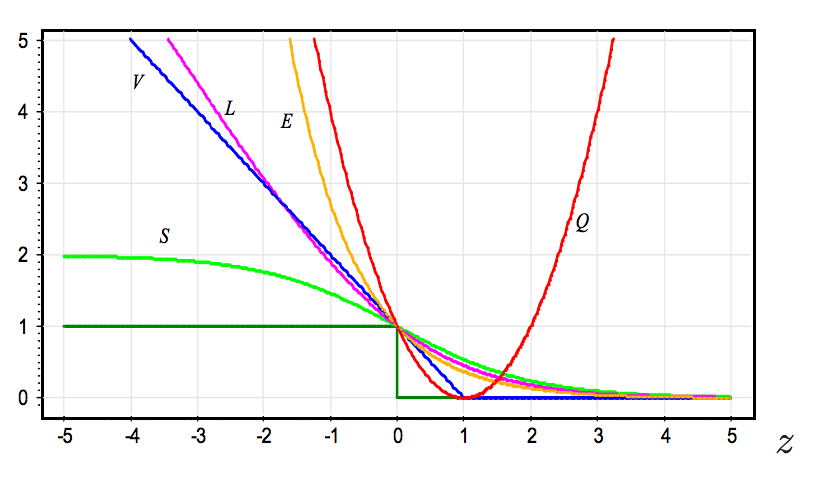
\includegraphics[width = 5in]{fig/approx.png}
\captionsetup{singlelinecheck=off}
\caption[]{Гладкие верхние аппроксимации пороговой функции потерь $[z < 0]$:
\begin{itemize}
  \item[] $S(z) = 2(1 + \exp(z))^{-1}$ --- сигмоидная;
  \item[] $L(z) = \log_{2} (1 + \exp(-z))$ --- логарифмическая;
  \item[] $V(z) = (1 - z)_+$ --- кусочно-линейная; 
  \item[] $E(z) = \exp(-z)$ --- экспоненциальная;
  \item[] $Q(z) = (1 - z)^2$ --- квадратичная.
\end{itemize}}
\label{fig:approx}
\end{figure}
 
\newpage
Алгоритм AdaBoost использует экспоненциальную аппроксимацию. Оценка функционал $Q_T$ сверху имеет вид:
  
  $ Q_T \leq \tilde Q_T = \sum \limits _{i = 1} ^ n \underset{u_i}{\underbrace{exp\{-y_i\sum\limits_{t=1}^{T-1}\omega_tb_t(x_i)}\}} exp\{-y_i\omega_Tb_T(x_i)\}$.

Введём вектор нормированных весов объектов $\tilde  V_n = (\tilde v_1,\dots,\tilde v_n), \tilde  v_i =  v_i / \sum \limits _{j = 1}^n v_j$.

Далее определим два функционала качества алгоритма классификации $b$ на обучающей выборке $X^n, Y^n$
с нормированным вектором весов объектов $U_n = (u_1 \dots,u_n)$ --- суммарный вес ошибочных (negative)  классификаций $N(b;U_n)$ и суммарный вес верных (positive) классификаций $P(b; U_n)$:

$N(b, U_n) = \sum\limits_{i = 1}^n  u_i[b(x_i) = -y_i], \quad P(b, U_n) = \sum\limits_{i = 1}^n  u_i[b(x_i) = y_i].$ 

Стоит отметить, что при отсутствии отказов алгоритма от классификации, $N + P = 1$.

\textbf{Теорема 1(Freund, Schapire, 1996).} Пусть для любого нормированного вектора весов $ U_n$ существует алгоритм $b \in \mathcal{B}$: $P(b, U_n) > N(b, U_n)$. \\
 Тогда минимум функционала $\tilde Q_T$ достигается при 
 
 $b_T =  \underset{b  \in \mathcal{B}}{\arg\max} \sqrt{P(b;\tilde V_n)} - \sqrt{N(b;\tilde V_n)}$, $\omega_T = \frac{1}{2} \ln\frac{P(b_T,\tilde V_n)}{N(b_T,\tilde V_n)}$.

Пусть $b_t: X \rightarrow \{-1;+1\}$. Тогда $P = 1 - N$.

\textbf{Теорема 2(Freund, Schapire, 1995).} Пусть для любого нормированного вектора весов $ V_n$ существует алгоритм $b \in \mathcal{B}$: $N(b, V_n) < \frac{1}{2}$.
 Тогда минимум функционала $\tilde Q_T$ достигается при  
 $b_T =  \underset{b  \in \mathcal{B}}{\arg\min} N(b;\tilde U_n)$, $\omega_T = \frac{1}{2} \ln\frac{1 - N(b_T,\tilde U_n)}{N(b_T,\tilde U_n)}$.

\subsection*{Алгоритм AdaBoost}

{\bf {Вход}}: $X^n, T$.

{\bf {Выход}}: $\omega_t, b_t, t = 1,\dots,T$.
\begin{enumerate}
    \item $u_i := 1/n, i = 1,\dots,n$;
    \item для всех $t = 1,\dots,T$
    \item обучить базовый алгоритм: $b_T =  \underset{b  \in \mathcal{B}}{\arg\min} N(b;\tilde U_n)$; 
    \item $\omega_T = \frac{1}{2} \ln\frac{1 - N(b_T,\tilde U_n)}{N(b_T,\tilde U_n)}$;
    \item пересчитать веса объектов $u_i := u_i \exp\{-\omega_t y_i b_t(x_i)\}, i = 1,\dots,n$;
    \item нормировать веса объектов: $u_0 := \sum\limits_{j=1}^n u_i$; $u_i := u_i/u_0, i = 1,\dots,n$;
\end{enumerate}

\section{Градиентный бустинг}

\section{Стохастический бустинг}
\end{document}
